\section{Aplikasi dalam Lexical Analysis}

Gambar \ref{fig:lexical-pipeline} menunjukkan alur lengkap dari regular expression hingga token recognition dalam lexical analysis.

\begin{figure}[H]
    \centering
    \adjustbox{max width=0.9\textwidth,center}{%
    \begin{tikzpicture}[
        box/.style={rectangle, draw=blue!50, fill=blue!10, text width=2.2cm, text centered, minimum height=0.8cm, rounded corners, font=\footnotesize, inner sep=4pt, align=center},
        arrow/.style={->, >=stealth, thick},
        node distance=1.5cm
    ]
    
    \node[box] (regex) {Regular\\Expressions};
    \node[box, right=of regex] (nfa) {NFA\\(Thompson)};
    \node[box, right=of nfa] (dfa) {DFA\\(Subset)};
    \node[box, right=of dfa] (min) {Minimized\\DFA};
    \node[box, right=of min] (scan) {Token\\Scanner};
    
    \draw[arrow] (regex) -- node[above, font=\tiny] {Konversi} (nfa);
    \draw[arrow] (nfa) -- node[above, font=\tiny] {Konversi} (dfa);
    \draw[arrow] (dfa) -- node[above, font=\tiny] {Optimasi} (min);
    \draw[arrow] (min) -- node[above, font=\tiny] {Simulasi} (scan);
    
    \end{tikzpicture}%
    }
    \caption{Alur proses dari regular expression ke token scanner}
    \label{fig:lexical-pipeline}
\end{figure}

\subsection{Token Recognition dengan DFA}

Dalam lexical analysis, kita menggunakan DFA untuk mengenali token. Prosesnya:

\begin{enumerate}
    \item \textbf{Definisi Token}: Setiap jenis token didefinisikan dengan regular expression
    \item \textbf{Kombinasi Regex}: Semua regex untuk token digabungkan dengan union
    \item \textbf{Konversi ke DFA}: Regex gabungan dikonversi menjadi satu DFA
    \item \textbf{Scanning}: Input dibaca karakter demi karakter, DFA dijalankan
    \item \textbf{Longest Match}: Ambil token terpanjang yang cocok
    \item \textbf{Token Classification}: Tentukan jenis token berdasarkan accept state yang dicapai
\end{enumerate}

\subsection{Contoh: Recognizer untuk Identifier dan Number}

Mari kita buat recognizer sederhana untuk identifier dan number. Gambar \ref{fig:identifier-dfa} dan \ref{fig:number-dfa} menunjukkan DFA untuk masing-masing pattern.

\begin{figure}[H]
    \centering
    \adjustbox{max width=0.7\textwidth,center}{%
    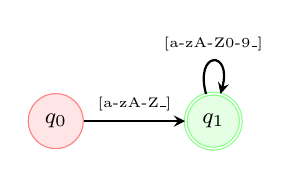
\begin{tikzpicture}[
        state/.style={circle, draw=blue!50, fill=blue!10, minimum size=0.7cm, font=\footnotesize},
        accept/.style={circle, draw=green!50, fill=green!10, minimum size=0.7cm, font=\footnotesize, double},
        start/.style={circle, draw=red!50, fill=red!10, minimum size=0.7cm, font=\footnotesize},
        arrow/.style={->, >=stealth, thick},
        node distance=2cm
    ]
    
    \node[start] (q0) at (0,0) {$q_0$};
    \node[accept] (q1) at (2,0) {$q_1$};
    
    \draw[arrow] (q0) -- node[above, font=\tiny] {[a-zA-Z\_]} (q1);
    \draw[arrow] (q1) to[loop above] node[above, font=\tiny] {[a-zA-Z0-9\_]} (q1);
    
    \end{tikzpicture}%
    }
    \caption{DFA untuk identifier: \texttt{[a-zA-Z\_][a-zA-Z0-9\_]*}}
    \label{fig:identifier-dfa}
\end{figure}

\begin{figure}[H]
    \centering
    \adjustbox{max width=0.5\textwidth,center}{%
    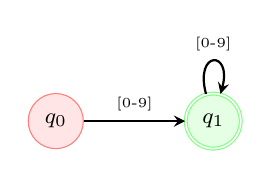
\begin{tikzpicture}[
        state/.style={circle, draw=blue!50, fill=blue!10, minimum size=0.7cm, font=\footnotesize},
        accept/.style={circle, draw=green!50, fill=green!10, minimum size=0.7cm, font=\footnotesize, double},
        start/.style={circle, draw=red!50, fill=red!10, minimum size=0.7cm, font=\footnotesize},
        arrow/.style={->, >=stealth, thick},
        node distance=2cm
    ]
    
    \node[start] (q0) at (0,0) {$q_0$};
    \node[accept] (q1) at (2,0) {$q_1$};
    
    \draw[arrow] (q0) -- node[above, font=\tiny] {[0-9]} (q1);
    \draw[arrow] (q1) to[loop above] node[above, font=\tiny] {[0-9]} (q1);
    
    \end{tikzpicture}%
    }
    \caption{DFA untuk number: \texttt{[0-9]+}}
    \label{fig:number-dfa}
\end{figure}

\begin{lstlisting}[language=C++, caption={Token Recognizer menggunakan DFA}]
enum TokenType {
    IDENTIFIER,
    NUMBER,
    UNKNOWN
};

class TokenRecognizer {
private:
    DFA identifier_dfa;  // DFA untuk [a-zA-Z_][a-zA-Z0-9_]*
    DFA number_dfa;      // DFA untuk [0-9]+
    
public:
    TokenRecognizer() {
        // Konstruksi DFA untuk identifier dan number
        // (dari regex menggunakan Thompson + subset construction)
        buildIdentifierDFA();
        buildNumberDFA();
    }
    
    TokenType recognize(const std::string& lexeme) {
        if (identifier_dfa.simulate(lexeme)) {
            return IDENTIFIER;
        } else if (number_dfa.simulate(lexeme)) {
            return NUMBER;
        } else {
            return UNKNOWN;
        }
    }
    
private:
    void buildIdentifierDFA() {
        // Implementasi konstruksi DFA untuk identifier
        // Regex: [a-zA-Z_][a-zA-Z0-9_]*
    }
    
    void buildNumberDFA() {
        // Implementasi konstruksi DFA untuk number
        // Regex: [0-9]+
    }
};
\end{lstlisting}

Contoh penggunaan:

\begin{lstlisting}[language=C++, caption={Contoh penggunaan TokenRecognizer}]
int main() {
    TokenRecognizer recognizer;
    
    std::vector<std::string> test_inputs = {
        "variable123",  // IDENTIFIER
        "42",           // NUMBER
        "_private",     // IDENTIFIER
        "3.14",         // UNKNOWN (belum support float)
        "123abc"        // UNKNOWN (mixed)
    };
    
    for (const auto& input : test_inputs) {
        TokenType type = recognizer.recognize(input);
        std::cout << input << " -> ";
        switch(type) {
            case IDENTIFIER: std::cout << "IDENTIFIER\n"; break;
            case NUMBER: std::cout << "NUMBER\n"; break;
            case UNKNOWN: std::cout << "UNKNOWN\n"; break;
        }
    }
    
    return 0;
}
\end{lstlisting}

\subsection{Handling Multiple Tokens}

Ketika kita memiliki multiple token types, kita perlu menggabungkan semua pattern menjadi satu DFA. Gambar \ref{fig:multiple-tokens} menunjukkan proses penggabungan NFA untuk multiple token types.

\begin{figure}[H]
    \centering
    \adjustbox{max width=0.85\textwidth,center}{%
    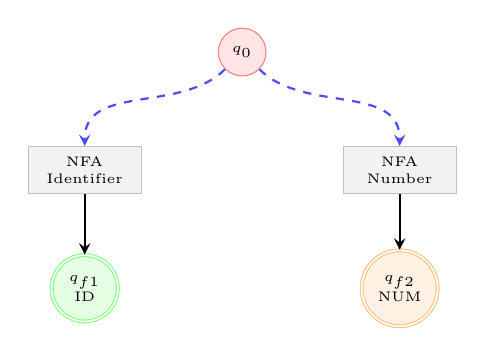
\begin{tikzpicture}[
        state/.style={circle, draw=blue!50, fill=blue!10, minimum size=0.6cm, font=\tiny},
        accept1/.style={circle, draw=green!50, fill=green!10, minimum size=0.6cm, font=\tiny, double, align=center},
        accept2/.style={circle, draw=orange!50, fill=orange!10, minimum size=0.6cm, font=\tiny, double, align=center},
        start/.style={circle, draw=red!50, fill=red!10, minimum size=0.6cm, font=\tiny},
        box/.style={rectangle, draw=gray!50, fill=gray!10, text width=1.2cm, minimum height=0.6cm, font=\tiny, align=center},
        arrow/.style={->, >=stealth, thick},
        eps/.style={->, >=stealth, thick, dashed, blue!70},
        node distance=1.2cm
    ]
    
    \node[start] (q0) at (0,0) {$q_0$};
    \node[box] (nfa1) at (-2,-1.5) {NFA\\Identifier};
    \node[box] (nfa2) at (2,-1.5) {NFA\\Number};
    \node[accept1] (qf1) at (-2,-3) {$q_{f1}$\\ID};
    \node[accept2] (qf2) at (2,-3) {$q_{f2}$\\NUM};
    
    \draw[eps] (q0) to[out=225, in=90] (nfa1);
    \draw[eps] (q0) to[out=315, in=90] (nfa2);
    \draw[arrow] (nfa1) -- (qf1);
    \draw[arrow] (nfa2) -- (qf2);
    
    \end{tikzpicture}%
    }
    \caption{Penggabungan NFA untuk multiple token types dengan labeling accept states}
    \label{fig:multiple-tokens}
\end{figure}

Proses handling multiple tokens:

\begin{enumerate}
    \item Membuat NFA terpisah untuk setiap token type
    \item Menggabungkan semua NFA dengan union, tetapi \textbf{label setiap accept state} dengan token type-nya
    \item Konversi ke DFA (setiap DFA state mungkin mengandung multiple NFA accept states dengan label berbeda)
    \item Saat scanning, jika mencapai accept state dengan multiple labels, gunakan \textbf{priority} atau \textbf{longest match}
\end{enumerate}

Contoh implementasi untuk multiple tokens:

\begin{lstlisting}[language=C++, caption={Handling Multiple Token Types}]
class MultiTokenRecognizer {
private:
    DFA combined_dfa;
    std::map<int, TokenType> state_to_token;
    
public:
    TokenType recognize(const std::string& lexeme) {
        int final_state = combined_dfa.simulate(lexeme);
        if (final_state == -1) return UNKNOWN;
        
        // Jika state memiliki multiple labels, gunakan priority
        if (state_to_token.find(final_state) != state_to_token.end()) {
            return state_to_token[final_state];
        }
        return UNKNOWN;
    }
    
    // Longest match: scan sampai tidak bisa lanjut
    Token scanLongestMatch(std::istream& input) {
        std::string lexeme;
        int last_accept_state = -1;
        int last_accept_pos = -1;
        int current_state = start_state;
        int pos = 0;
        
        char c;
        while (input.get(c)) {
            lexeme += c;
            // Update state dengan input c
            // ...
            
            if (isAcceptState(current_state)) {
                last_accept_state = current_state;
                last_accept_pos = pos;
            }
            pos++;
        }
        
        // Kembalikan ke posisi terakhir yang accept
        input.seekg(last_accept_pos);
        return Token(state_to_token[last_accept_state], 
                     lexeme.substr(0, last_accept_pos + 1));
    }
};
\end{lstlisting}